\section{Introduction}\label{introduction}

High-resolution animal tracking has made migration analysis increasingly curve based rather than point based. Individual tracks can now be compared as routes, clustered into broad movement patterns, and screened for unusual trajectories \citep{kranstauber2011, kays2022}. These analyses depend on distance matrices computed from movement paths. In practice, however, tracking records are rarely complete. Devices can fail temporarily, transmission schedules may be irregular, and long movements can contain prolonged gaps. When these gaps are collapsed into one completed route, downstream conclusions can appear more stable than the data justify.

Most route-comparison pipelines handle missing observations by preprocessing each track into one deterministic curve. Sparse or interrupted records may be resampled, interpolated, or trimmed before a trajectory distance is computed. This is computationally convenient, but it hides a methodological distinction between two types of incompleteness. Randomly missing points along an otherwise observed route may be largely absorbed by resampling. A contiguous gap during active migration is different: the unobserved segment may contain a substantial portion of the route geometry. The distance between two reconstructed routes, and therefore any clustering or anomaly score based on that distance, can depend strongly on how the missing segment is filled.

The unresolved issue is therefore not only how to reconstruct a missing segment, but how reconstruction uncertainty affects the route-comparison conclusions that analysts actually use. This paper asks how uncertainty from prolonged tracking gaps propagates into migratory-route comparison. The contribution is an ecological-informatics diagnostic framework for validating, calibrating, and propagating missing-route uncertainty: remove observations under controlled missingness mechanisms, reconstruct plausible missing route segments, check uncertainty envelopes against withheld observations, calibrate those envelopes when needed, and measure whether downstream conclusions remain stable.

The empirical case study uses open GPS tracking data for Lesser Black-backed Gulls (\emph{Larus fuscus}). Candidate migration routes are embedded on the unit sphere and compared using two aligned trajectory metrics: raw-coordinate dynamic time warping (DTW) and DTW-aligned square root velocity function distance (SRVF-DTW). These metrics are treated as downstream analysis tools rather than as the novelty of the paper. The aim is not to introduce a new trajectory distance or to claim new biological findings about gull migration. The central question is whether the resulting distance matrices, route clusters, and anomaly rankings are robust to plausible reconstructions of missing route segments.

The case study is not intended to support species-general biological conclusions about gull migration. It is used because the dataset is open, large, and reproducible enough to demonstrate the diagnostic sequence end to end. The transferable component is the problem-solution structure: define route units, impose controlled missingness, reconstruct plausible missing segments, validate and calibrate their uncertainty envelopes when withheld observations are available, and propagate the resulting uncertainty into downstream route-comparison outputs.

The contributions are:

\begin{enumerate}
\def\labelenumi{\arabic{enumi}.}
\tightlist
\item A controlled comparison of random point loss and contiguous tracking gaps in migratory-route distance analysis.
\item Evidence that deterministic spherical bridge interpolation does not fully resolve the instability introduced by prolonged gaps.
\item A movement-aware Brownian bridge baseline that samples plausible missing route segments on the unit sphere.
\item Season-specific estimation of Brownian bridge perturbation scales from observed local route residuals.
\item Withheld-segment validation and empirical radius-inflation calibration for checking whether sampled missing-route envelopes achieve nominal coverage.
\item Propagation of reconstruction uncertainty into distance-matrix rank correlation, relative distance error, clustering agreement, anomaly-rank correlation, and top-ranked anomaly overlap.
\end{enumerate}

\section{Data and Route Construction}\label{data-and-route-construction}

The empirical analysis uses the open \texttt{LBBG\_ZEEBRUGGE} dataset published by the Research Institute for Nature and Forest (INBO) \citep{stienen2025}. The dataset contains GPS tracking records for Lesser Black-backed Gulls breeding near the southern North Sea coast and is distributed as a Darwin Core Archive under a CC0 1.0 license. The version used here is version 1.3, published on 25 August 2025.

The Darwin Core occurrence table contains 1,801,214 records. After filtering to GPS events with valid individual identifiers, timestamps, and coordinates, 1,801,052 standardized GPS records were retained. Records were grouped by individual and sorted chronologically. The raw data include breeding-area movement, stopovers, wintering-area movement, and repeated annual cycles, so full individual time series were not used directly as route-comparison units.

Candidate migration segments were extracted with a transparent seasonal heuristic. Spring candidate segments used February to May records, and autumn candidate segments used July to November records. Distances were computed from an approximate Zeebrugge breeding-colony reference point at 51.34\(^\circ\)N, 3.18\(^\circ\)E. Segments were retained when they contained at least 30 GPS points, reached at least 300 km from this reference point, and had a start-end displacement of at least 150 km. A transit-focused trimming step then reduced residence-period movement. Autumn routes were retained from first movement beyond 100 km from the colony until the route reached at least 90\% of its seasonal maximum distance. Spring routes were retained from departure from the distant wintering region until return within 100 km of the colony. Segments with fewer than 20 retained points were excluded.

This procedure produced 381 transit-focused candidate migration segments containing 374,341 GPS points. Table~\ref{tab:route-counts} summarizes the route counts by season and the balanced subset used in the season-aware Brownian bridge experiment. Figure~\ref{fig:route-overview-season} shows the seasonal route geometry used in the case study. The segmentation is intended as a reproducible route-extraction rule, not as a validated behavioral-state classifier.

A threshold sensitivity check was used to assess whether the candidate-route sample depended strongly on one trimming setting. Varying the departure/return threshold from 75 km to 150 km and the near-maximum-distance fraction from 0.85 to 0.95 retained 377 to 383 total transit routes, compared with 381 under the baseline rule. The retained point count varied more substantially, from 272,794 to 413,853 points, reflecting different amounts of residence-period movement kept near route endpoints. This supports using the rule as a stable candidate-route extraction procedure while reinforcing that the exact start and end times should not be interpreted as validated behavioral-state transitions.

\begin{table}[H]
\centering
\caption{Route counts after broad seasonal filtering and transit-focused trimming. The Brownian bridge batch experiment used a balanced subset of 30 transit routes per season.}
\label{tab:route-counts}
\resizebox{\textwidth}{!}{%
\begin{tabular}{lrrrrr}
\toprule
Season & Broad routes & Transit routes & Individuals & Transit points & Batch routes \\
\midrule
Spring & 204 & 200 & 84 & 74,567 & 30 \\
Autumn & 182 & 181 & 81 & 299,774 & 30 \\
Total & 386 & 381 & 88 & 374,341 & 60 \\
\bottomrule
\end{tabular}
}
\end{table}

\begin{figure}[t]
\centering
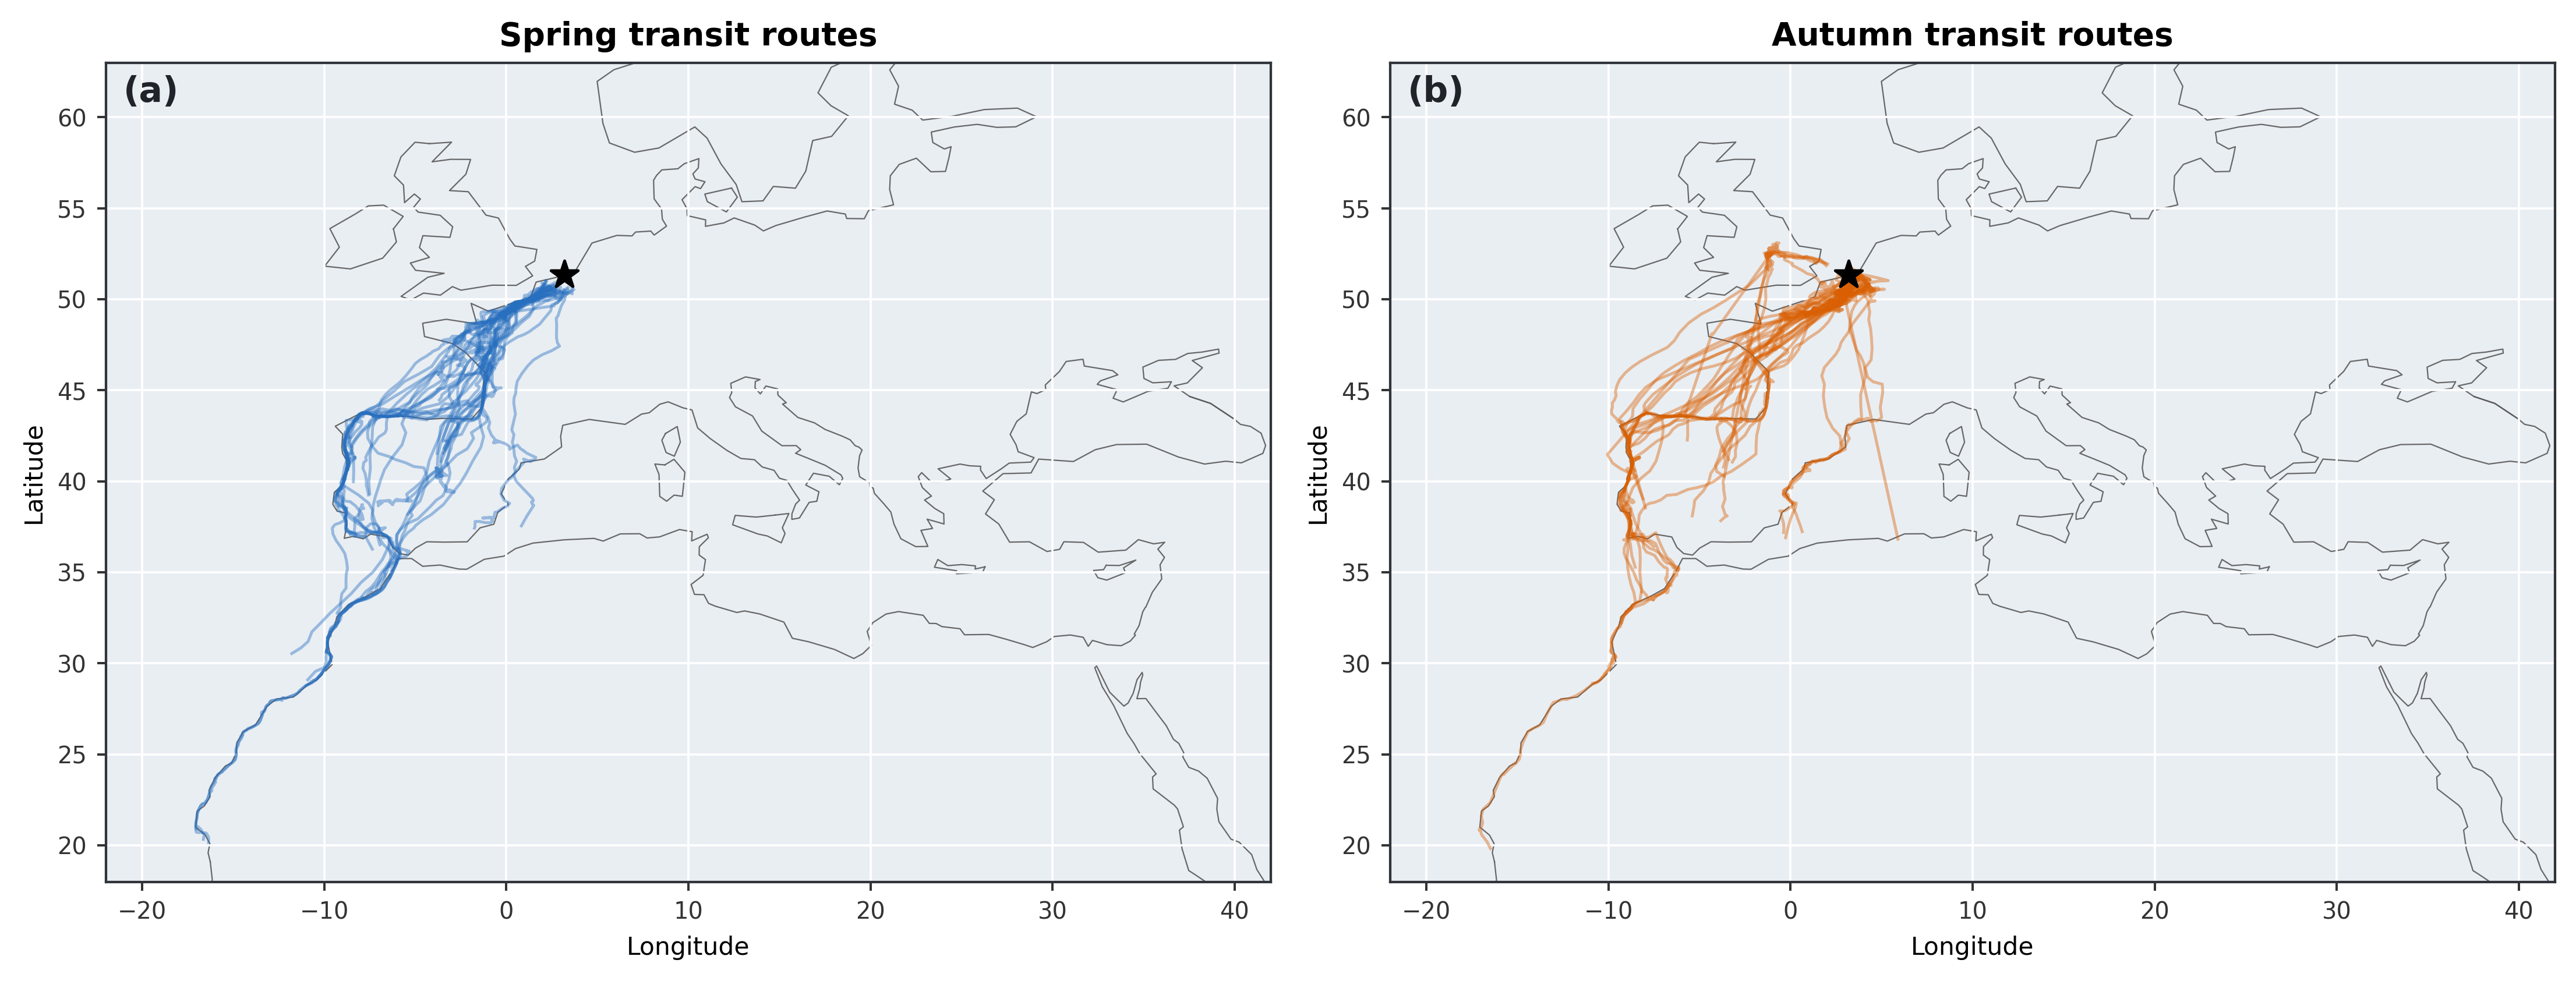
\includegraphics[width=\textwidth]{../../figures/route_overview_by_season.png}
\caption{Seasonal overview of transit-focused Lesser Black-backed Gull migration routes used in the case study. Spring and autumn route sets are shown separately to emphasize that missing-route uncertainty was evaluated across season-specific movement geometry rather than on a single pooled track set.}
\label{fig:route-overview-season}
\end{figure}

\section{Methods}\label{methods}

\subsection{Diagnostic Design}\label{diagnostic-design}

The analysis was organized as a validate--calibrate--propagate diagnostic rather than as a single reconstruction procedure. First, complete observed routes were represented in a common spherical coordinate system and compared with two trajectory-distance metrics. Second, controlled missingness mechanisms were imposed to separate random point loss from prolonged contiguous gaps. Third, deterministic and stochastic gap-reconstruction baselines were applied to the incomplete routes. Fourth, Brownian bridge uncertainty envelopes were validated against withheld observed route segments and empirically calibrated when nominal coverage was not achieved. Finally, the resulting reconstruction uncertainty was propagated into the downstream outputs normally used in route-comparison studies: distance matrices, cluster labels, anomaly rankings, and top-ranked anomaly overlap.

\begin{table}[H]
\centering
\caption{Validate--calibrate--propagate workflow used in the manuscript.}
\label{tab:diagnostic-workflow}
\small
\begin{tabular}{p{0.28\textwidth}p{0.62\textwidth}}
\toprule
Step & Diagnostic purpose \\
\midrule
Define route units & Extract reproducible transit-focused candidate routes and represent them on the unit sphere. \\
Impose missingness & Compare random point loss with prolonged contiguous tracking gaps under controlled removal fractions. \\
Reconstruct gaps & Apply deterministic spherical bridges and stochastic Brownian bridge samples to incomplete routes. \\
Validate envelopes & Check Brownian sample envelopes against withheld observed route segments. \\
Calibrate coverage & Estimate empirical radius inflation when nominal 90\% envelopes are too narrow. \\
Propagate uncertainty & Recompute route distances, cluster labels, anomaly rankings, and top-ranked anomaly overlap under reconstructed routes. \\
\bottomrule
\end{tabular}
\end{table}

\subsection{Spherical Route Representation}\label{spherical-route-representation}

Latitude-longitude coordinates were embedded into the three-dimensional unit sphere. For latitude \(\phi\) and longitude \(\lambda\), both in radians, each observation was transformed as

\[
x = \cos(\phi)\cos(\lambda), \quad
y = \cos(\phi)\sin(\lambda), \quad
z = \sin(\phi).
\]

Each route was resampled to a fixed number of points using chord-length interpolation in the embedded coordinate system, followed by normalization back to the unit sphere. This representation avoids treating long-distance routes as planar longitude-latitude curves and gives a common discretization for distance computation. The resulting route representation is

\[
P_i = \{p_{i1}, \ldots, p_{im}\}, \quad p_{it} \in S^2 \subset \mathbb{R}^3,
\]

where \(m\) is the common number of resampled points and \(S^2\) is the unit sphere.

\subsection{Route Metrics}\label{route-metrics}

Two aligned trajectory metrics were used as downstream diagnostics. Raw-coordinate DTW was applied directly to sampled unit-sphere coordinate sequences. DTW addresses traversal-timing variation by aligning point sequences through dynamic programming \citep{sakoe1978}. For two route sequences \(P_i\) and \(P_j\), the raw-DTW distance was written as

\[
d_{\mathrm{DTW}}(P_i,P_j)
= \min_{\pi \in \Pi}
\left(\sum_{(a,b)\in \pi} \lVert p_{ia}-p_{jb}\rVert_2^2\right)^{1/2},
\]

where \(\Pi\) is the set of monotone admissible warping paths. SRVF-DTW was computed by first converting each sampled route to a discrete square root velocity function representation and then applying DTW to the resulting vector-valued sequence \citep{srivastava2011}. For a curve \(f(t)\), the SRVF is

\[
q(t) = \frac{\dot f(t)}{\sqrt{\|\dot f(t)\|}}.
\]

For sampled routes, this produced SRVF sequences \(Q_i=\{q_{i1},\ldots,q_{i,m-1}\}\), and \(d_{\mathrm{SRVF\text{-}DTW}}(P_i,P_j)=d_{\mathrm{DTW}}(Q_i,Q_j)\). Raw-coordinate DTW and SRVF-DTW represent two different views of route similarity. Raw DTW emphasizes spatial alignment of geographic corridors. SRVF-DTW emphasizes aligned local velocity-shape structure. In this paper, they are not compared to establish a universally superior metric. They are used to test whether uncertainty from missing route segments changes downstream route-comparison conclusions.

\subsection{Missingness Experiments}\label{missingness-experiments}

Two missingness mechanisms were evaluated. In the random point-loss experiment, 20\%, 40\%, or 60\% of observations were removed at random from each route before resampling and distance computation. In the contiguous-gap experiment, one continuous block covering 20\%, 40\%, or 60\% of each route was removed. Each condition was repeated five times.

For each incomplete dataset, raw-DTW and SRVF-DTW distance matrices were recomputed and compared with the complete-route baseline. Stability was measured with five diagnostics: Spearman correlation between upper triangles of the distance matrices, median relative distance error, adjusted Rand index for agglomerative cluster labels, Spearman correlation of anomaly scores, and overlap among the top-ranked anomalous routes.

\subsection{Gap Reconstruction Baselines}\label{gap-reconstruction-baselines}

The first reconstruction baseline was deterministic spherical bridge interpolation. The missing segment endpoints were connected by spherical interpolation, and the reconstructed route was then resampled. This baseline represents a common implicit assumption: the unobserved segment is replaced by one smooth path between the observed endpoints.

The uncertainty-aware baseline was a tangent-plane Brownian bridge, motivated by Brownian bridge movement models used to represent uncertainty between observed animal locations \citep{horne2007}. For each missing interval, a deterministic spherical bridge supplied the mean path \(m(t)\) between the endpoints, with \(t\in[0,1]\). A sampled missing point was generated as

\[
\tilde p^{(b)}(t)
= \frac{m(t) + \sigma E(t) z^{(b)}(t)}
{\lVert m(t) + \sigma E(t) z^{(b)}(t)\rVert_2},
\]

where \(E(t)\) is a local two-dimensional tangent-plane basis at \(m(t)\), \(\sigma\) is the perturbation scale, and \(z^{(b)}(t)\) is a Brownian-bridge perturbation constrained to be zero at \(t=0\) and \(t=1\). In the implementation, the perturbation variance was proportional to \(t(1-t)\), so uncertainty was smallest at observed endpoints and largest inside the gap. The perturbation scale was estimated from observed local great-circle residuals. In the season-aware batch experiment, this scale was estimated separately for spring and autumn routes.

The Brownian bridge is used here as a practical baseline rather than a complete movement model. It does not condition on wind, habitat, stopover behavior, or individual movement state. Its purpose is to expose how plausible uncertainty inside missing intervals can affect the route-comparison outputs that ecologists may inspect.

\subsection{Withheld-Segment Validation}\label{withheld-segment-validation-methods}

A lightweight withheld-segment validation was used to check the reconstruction baselines against observed route geometry. For spring and autumn separately, 12 transit routes with at least 100 observations were selected. Continuous observed segments covering 20\%, 40\%, or 60\% of each route were withheld twice per condition. Deterministic spherical bridges and 12 Brownian bridge samples were then compared with the withheld observations at the original point locations.

Validation diagnostics included mean great-circle error, the error of the pointwise Brownian sample center, the best sampled-path error at each withheld point, and empirical coverage of a pointwise 90\% Brownian sample envelope. Let \(y_\ell\) denote a withheld observed point, \(\bar p_\ell\) the pointwise center of the Brownian samples, and \(r_\ell^{0.90}\) the empirical 90\% sample-envelope radius at that point. The pointwise error and uncalibrated coverage indicator were

\[
e_\ell = R \arccos(\bar p_\ell^\top y_\ell),
\quad
c_\ell^{0.90} = \mathbf{1}\{e_\ell \le r_\ell^{0.90}\},
\]

where \(R=6371\) km is the Earth radius. This validation was not intended to prove true-path recovery. Its purpose was to test whether the stochastic reconstruction envelope was wide enough to represent observed hidden route geometry at the stated nominal level.

\subsection{Empirical Envelope Calibration}\label{empirical-envelope-calibration}

To quantify calibration, the pointwise 90\% envelope radius was multiplied by the empirical 90th percentile of the ratio between withheld-point error and uncalibrated envelope radius:

\[
\alpha_{0.90}
= Q_{0.90}\left(\frac{e_\ell}{r_\ell^{0.90}+\epsilon}\right),
\quad
\tilde r_\ell^{0.90} = \alpha_{0.90} r_\ell^{0.90},
\]

where \(Q_{0.90}\) is the empirical 90th percentile and \(\epsilon\) is a small numerical constant. The calibrated pointwise coverage was

\[
\tilde C_{0.90}
= \frac{1}{L}\sum_{\ell=1}^{L}
\mathbf{1}\{e_\ell \le \tilde r_\ell^{0.90}\}.
\]

This radius-inflation factor estimates how much wider the Brownian envelope would need to be to approach nominal 90\% coverage on withheld observations. The calibrated envelope was then summarized by its achieved pointwise coverage and median calibrated radius. The calibration step is diagnostic: it reports the mismatch between the simple Brownian bridge envelope and withheld observations rather than claiming a universally valid correction factor.

\subsection{Uncertainty Propagation}\label{uncertainty-propagation-methods}

For each reconstructed route set, route distances were recomputed and compared with the complete-route baseline. Let \(D^{(0)}\) be the complete-route distance matrix and \(D^{(s)}\) the distance matrix from a missingness or reconstruction condition. Distance-matrix stability was measured as

\[
\rho_D = \rho_{\mathrm{S}}\{\operatorname{vec}_u(D^{(0)}),
\operatorname{vec}_u(D^{(s)})\},
\]

where \(\rho_{\mathrm{S}}\) is Spearman correlation and \(\operatorname{vec}_u(\cdot)\) extracts the upper triangle of a symmetric matrix. Median relative distance error was

\[
E_D =
\operatorname{median}_{i<j}
\frac{|D^{(s)}_{ij}-D^{(0)}_{ij}|}{D^{(0)}_{ij}+\epsilon}.
\]

Cluster stability was measured with adjusted Rand index between complete-route and reconstructed-route cluster labels. If \(a_i^{(0)}\) and \(a_i^{(s)}\) are anomaly scores derived from the corresponding distance matrices, anomaly-rank stability was

\[
\rho_A = \rho_{\mathrm{S}}(a^{(0)},a^{(s)}),
\quad
O_k = \frac{|T_k^{(0)}\cap T_k^{(s)}|}{k},
\]

where \(T_k\) is the set of the \(k\) highest-ranked anomalous routes. These outputs were chosen because they represent common downstream uses of route distances: comparing overall route similarity, grouping routes, and screening unusual trajectories. The same diagnostics were computed for observed-only incomplete routes, deterministic bridge reconstructions, and Brownian bridge samples so that reconstruction assumptions could be compared on the scale of downstream conclusions.

\subsection{Scale Sensitivity}\label{scale-sensitivity-methods}

Because the Brownian bridge perturbation scale is a simple empirical estimate, a lightweight scale-sensitivity check was also run. For 60\% contiguous gaps, the estimated seasonal scale was multiplied by 0.5, 1.0, and 2.0 in a small balanced subset of spring and autumn routes. This check was used to assess whether downstream conclusions changed smoothly with plausible scale inflation rather than depending on one fixed tuning value.

\section{Results}\label{results}

\subsection{Validate--Calibrate--Propagate Diagnostic}\label{validate-calibrate-propagate-diagnostic}

Figure~\ref{fig:uncertainty-framework} summarizes the proposed diagnostic. A contiguous tracking gap is introduced into an observed migration route, the missing interval is reconstructed either as a deterministic bridge or as a set of Brownian bridge samples, the sampled envelope is checked against withheld observations when available, and each reconstructed route is propagated through distance, clustering, and anomaly diagnostics.

\begin{figure}[t]
\centering
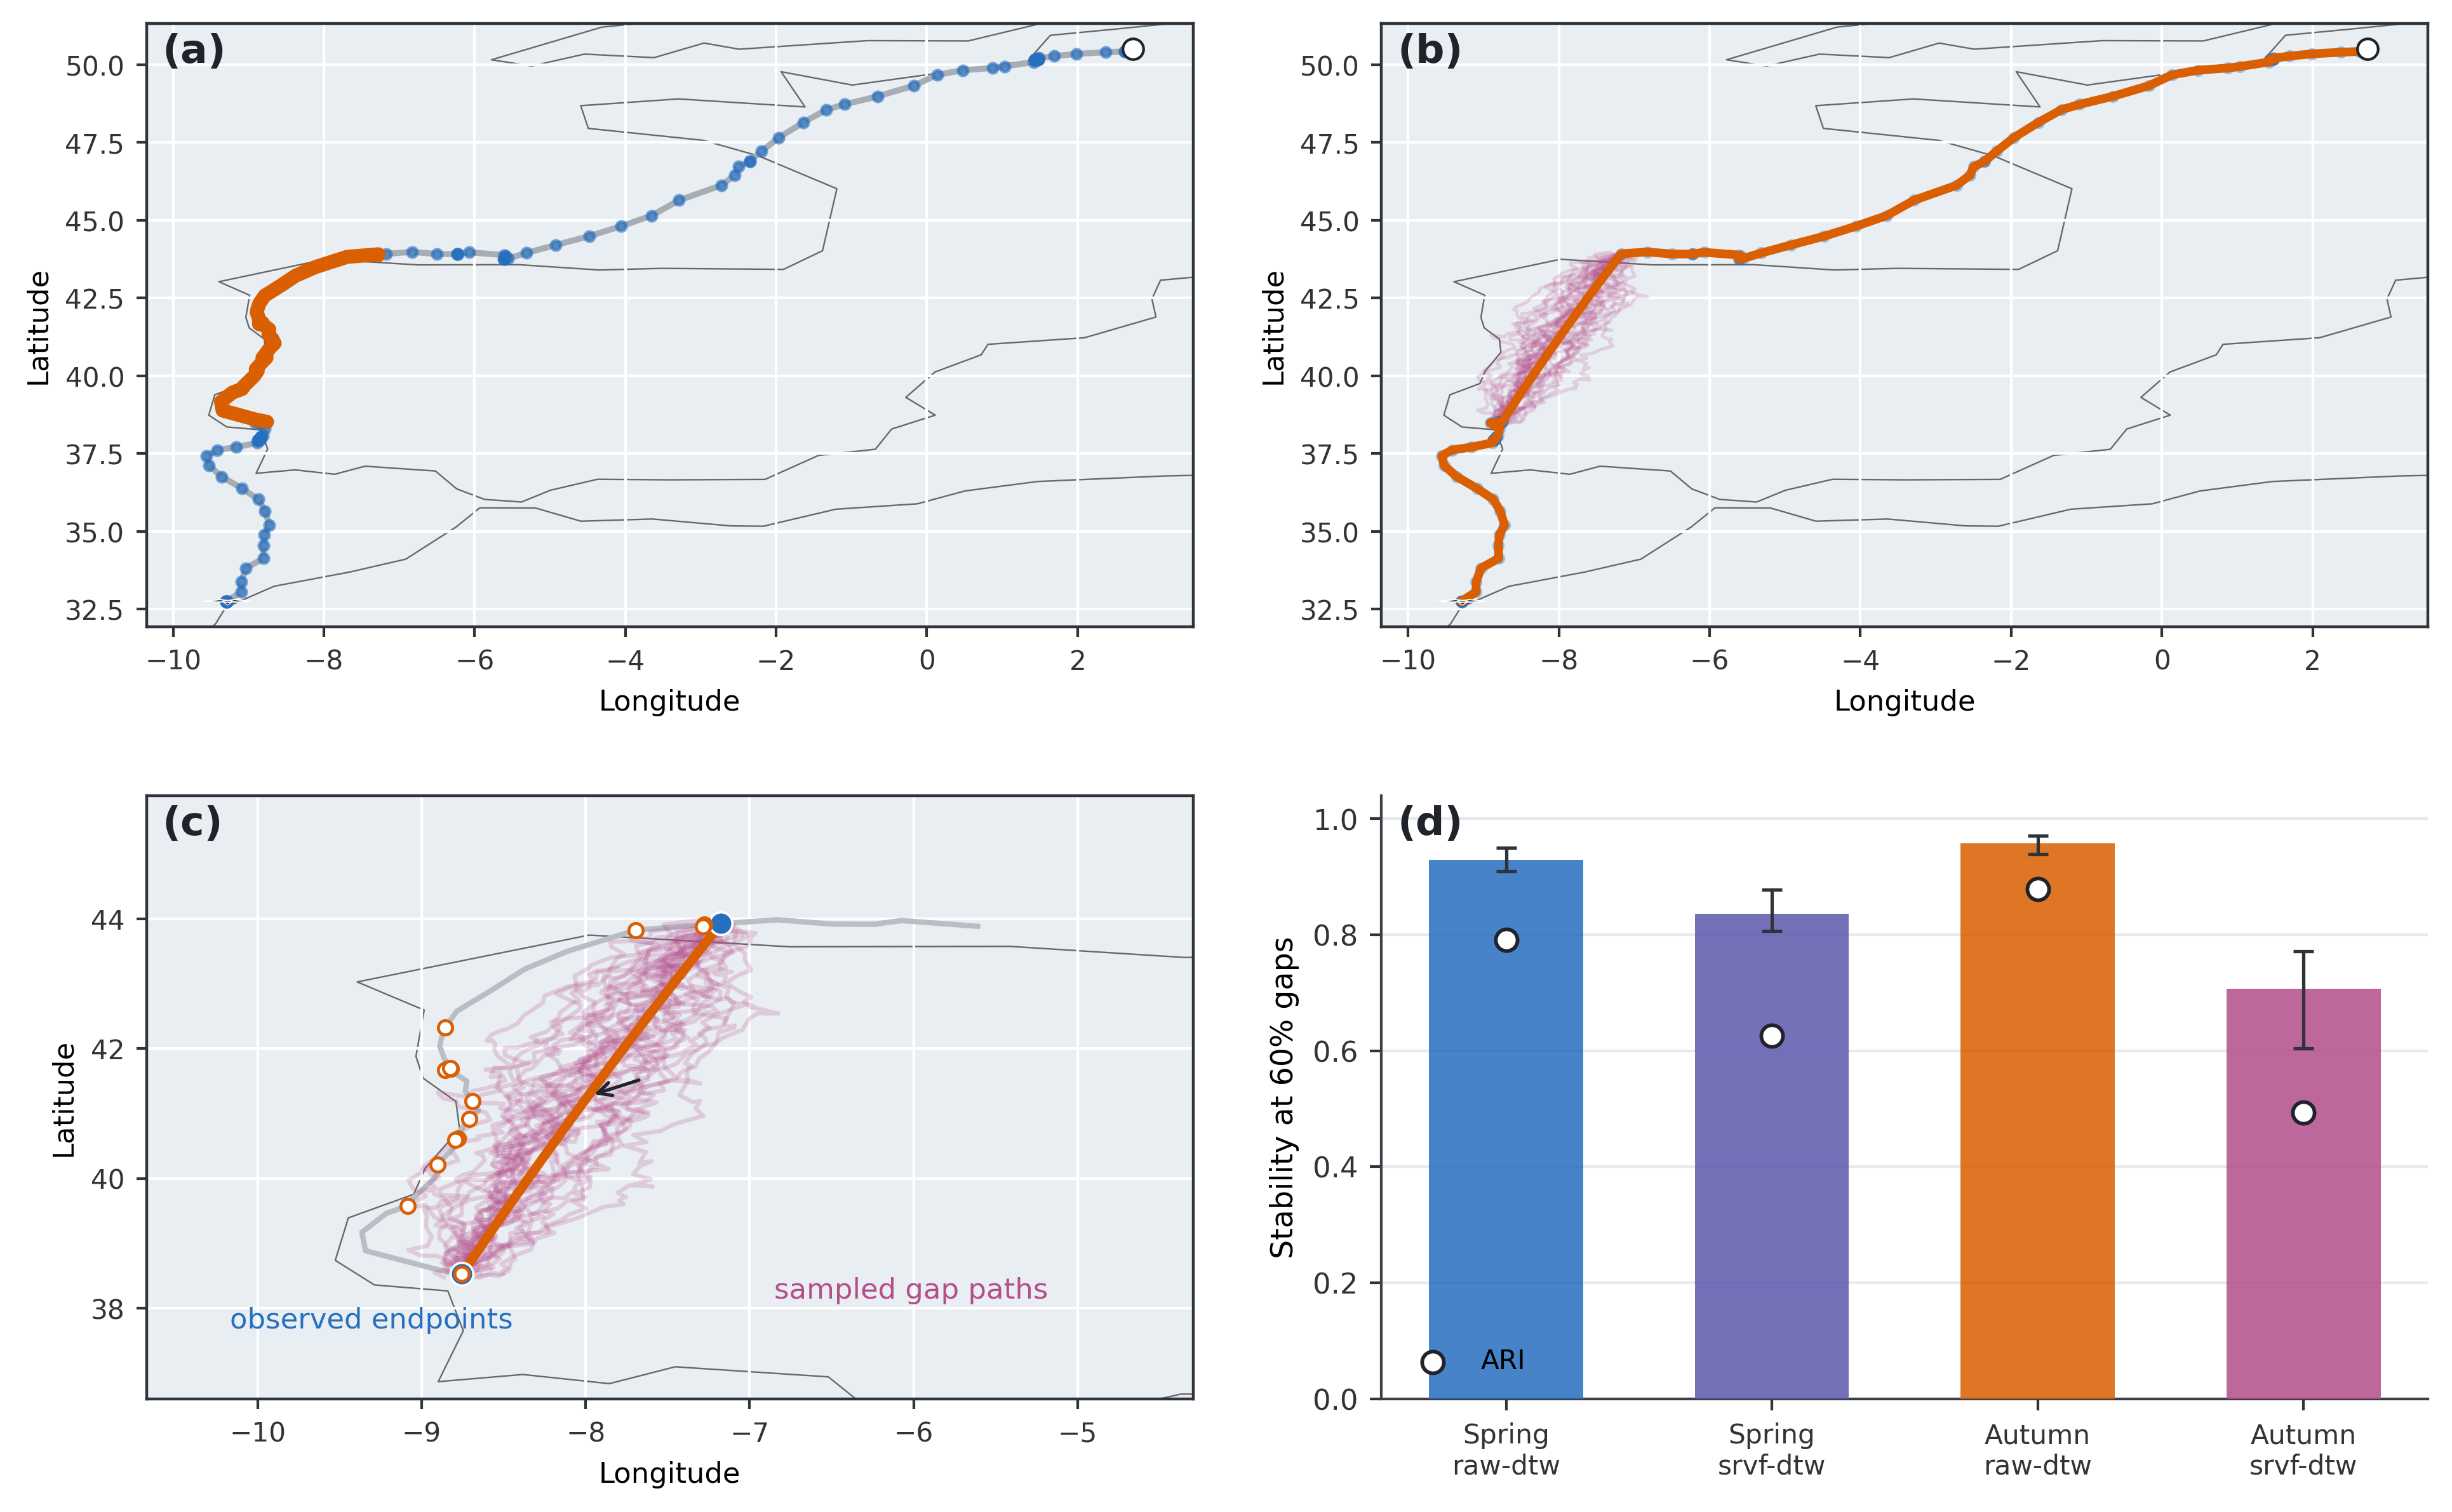
\includegraphics[width=\textwidth]{../../figures/route_gap_method_figure.png}
\caption{Route-gap uncertainty workflow and diagnostic outputs for incomplete animal tracking data. Panel (a) shows an observed migration route from a tracked bird, with the bird symbol marking the route start, the open circle marking the endpoint, and a contiguous withheld GPS gap highlighted. Panel (b) compares deterministic spherical-bridge reconstruction with stochastic Brownian bridge samples for the same missing interval. Panel (c) zooms into the missing interval and shows how observed endpoints define a spherical bridge while Brownian perturbations generate an ensemble of plausible missing-route paths. Panel (d) shows downstream stability at 60\% gaps, with distance-matrix rank correlation shown as bars and cluster agreement shown as points.}
\label{fig:uncertainty-framework}
\end{figure}

\subsection{Missingness Mechanism Matters}\label{missingness-mechanism-matters}

Random point loss had limited effect after route resampling. At 60\% random missingness, raw-DTW distance matrices remained almost unchanged, with mean matrix Spearman correlation 0.999 and median relative distance error 0.017. SRVF-DTW was more affected but still stable at the distance-matrix level, with mean matrix Spearman correlation 0.983 and median relative distance error 0.045.

Contiguous gaps produced larger instability. At 60\% contiguous missingness, raw-DTW matrix correlation decreased to 0.953, median relative distance error increased to 0.121, cluster agreement decreased to adjusted Rand index 0.569, and anomaly-rank correlation decreased to 0.869. For SRVF-DTW under the same condition, matrix correlation decreased to 0.884, median relative distance error increased to 0.211, cluster agreement decreased to 0.474, and anomaly-rank correlation was 0.906.

These results show that route-comparison stability depends on the missingness mechanism. Random thinning and prolonged tracking gaps should not be treated as equivalent data-quality problems. Figure~\ref{fig:missing-data-stability} summarizes these stability diagnostics across missingness mechanisms and route metrics.

\begin{figure}[t]
\centering
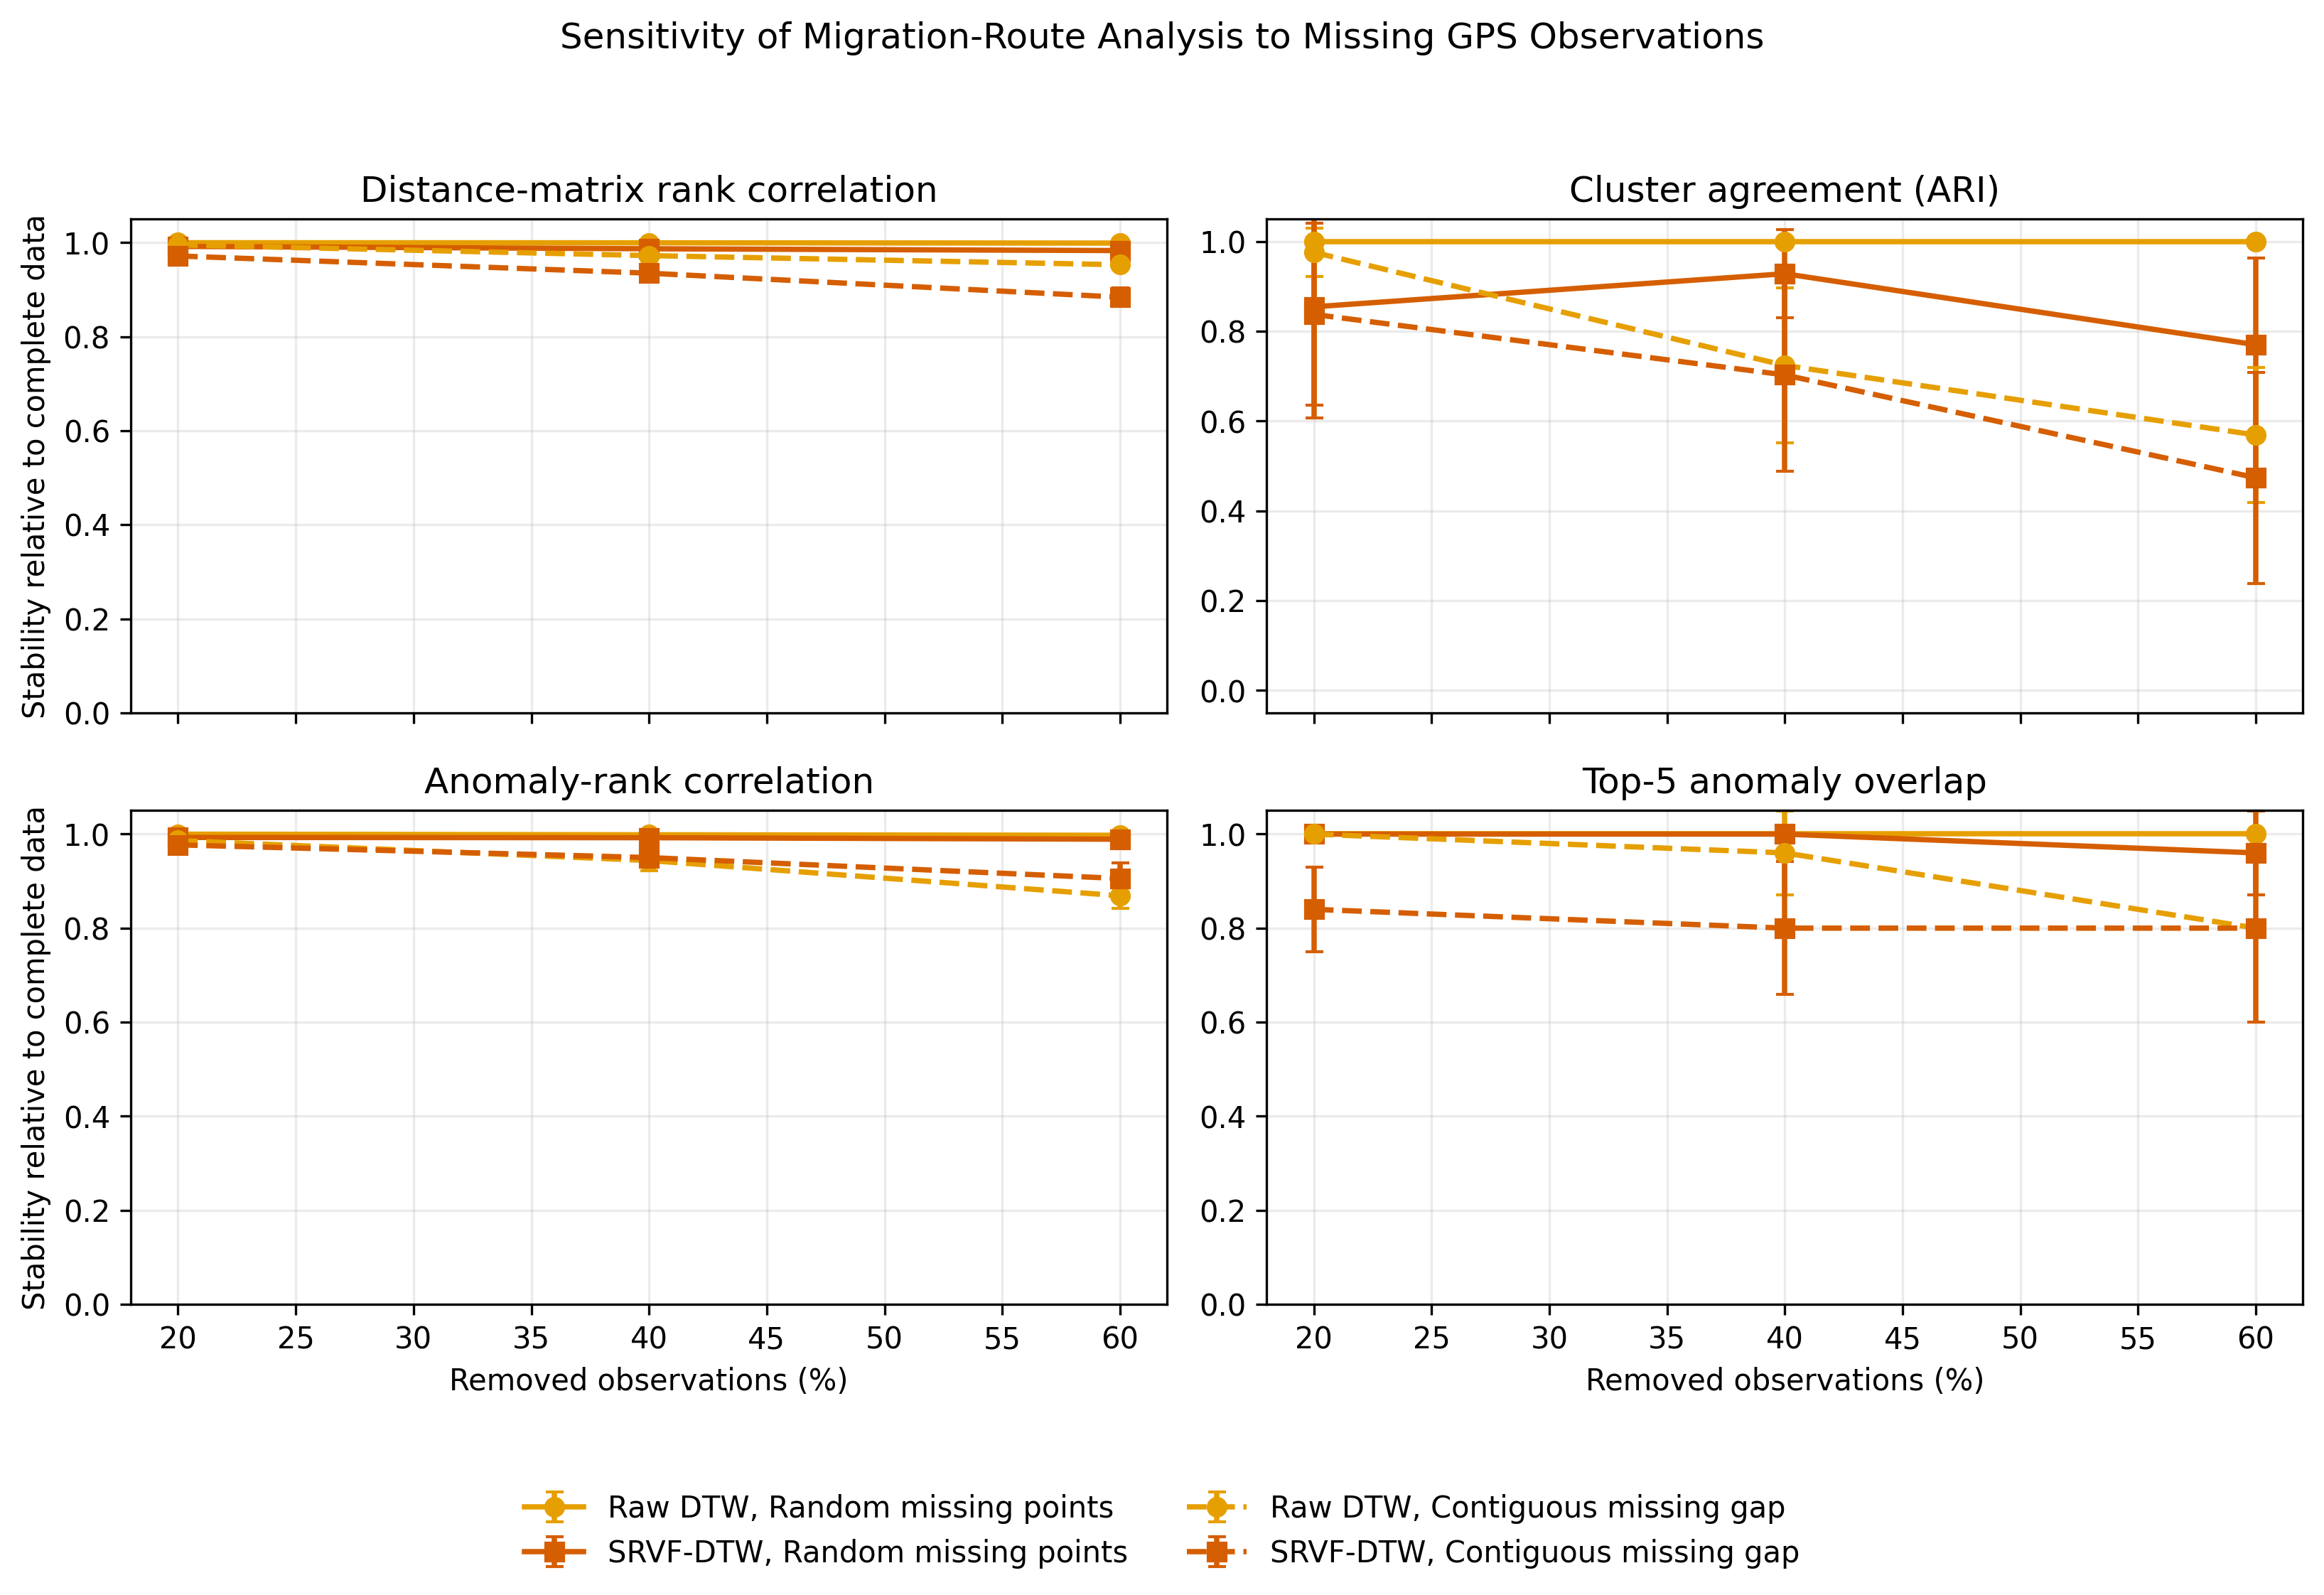
\includegraphics[width=\textwidth]{../../figures/missing_data_stability.png}
\caption{Stability of route-comparison diagnostics under random point loss and contiguous tracking gaps. Random point loss has limited effect after resampling, whereas contiguous gaps produce larger changes in distance matrices, clustering, and anomaly rankings.}
\label{fig:missing-data-stability}
\end{figure}

\subsection{Deterministic Interpolation Is Not Enough}\label{deterministic-interpolation-is-not-enough}

Spherical bridge interpolation did not fully recover the complete-data route-comparison structure. In the contiguous-gap baseline, observed-only resampling and deterministic spherical bridge reconstruction produced similar stability patterns. This indicates that replacing a gap with one smooth path between endpoints can leave the downstream analysis almost as sensitive as simply resampling the observed incomplete route.

The implication is practical. If a route has a long tracking gap, a single interpolated path should not be treated as if it were observed. Even when the reconstructed curve looks plausible, distance matrices and cluster assignments may still depend on the unobserved segment.

\subsection{Season-Aware Brownian Bridge Reconstruction}\label{season-aware-brownian-bridge-reconstruction}

The Brownian bridge experiment estimated movement perturbation scales from observed local route residuals. The estimated spring scale was 0.00108755, whereas the autumn scale was 0.000352488. This difference suggests that reconstruction uncertainty should not necessarily be shared across seasons.

In the season-aware batch experiment, 30 spring and 30 autumn transit routes were evaluated at 20\%, 40\%, and 60\% contiguous gap fractions. For each season and gap fraction, three repeated gap placements were generated, and six Brownian bridge samples were drawn per gap placement. Results showed that downstream stability depended on metric, season, and diagnostic. Raw-DTW distance-matrix correlations remained relatively high, while SRVF-DTW distance stability declined more strongly in some conditions. Cluster agreement was the least stable downstream conclusion. Anomaly rankings were often more stable than cluster labels, but they also degraded under severe gaps, especially for autumn SRVF-DTW.

At 60\% autumn gaps, Brownian bridge raw-DTW reconstructions had mean matrix correlation 0.958 and anomaly-rank correlation 0.931. Under SRVF-DTW, the corresponding values were 0.707 and 0.679. Figure~\ref{fig:brownian-bridge-batch} shows the full Brownian bridge diagnostic patterns across seasons, metrics, and gap fractions, and Table~\ref{tab:brownian-60} summarizes the corresponding 60\% gap diagnostics for both seasons and metrics. The difference does not imply that one metric is universally preferable. It shows that the effect of reconstruction uncertainty must be assessed for the specific downstream question and route representation.

A small scale-sensitivity check confirmed that this interpretation depends on the magnitude of assumed missing-route uncertainty. At 60\% gaps, doubling the estimated Brownian bridge scale reduced spring raw-DTW matrix correlation from 0.852 at the estimated scale to 0.616, and reduced autumn raw-DTW matrix correlation from 0.930 to 0.764. SRVF-DTW was more sensitive in autumn, where matrix correlation decreased from 0.574 at the estimated scale to 0.070 under the doubled scale. Figure~\ref{fig:brownian-scale-sensitivity} visualizes this scale dependence. The sensitivity check therefore supports reporting downstream diagnostics across plausible reconstruction scales when the bridge scale is uncertain.

\begin{figure}[t]
\centering
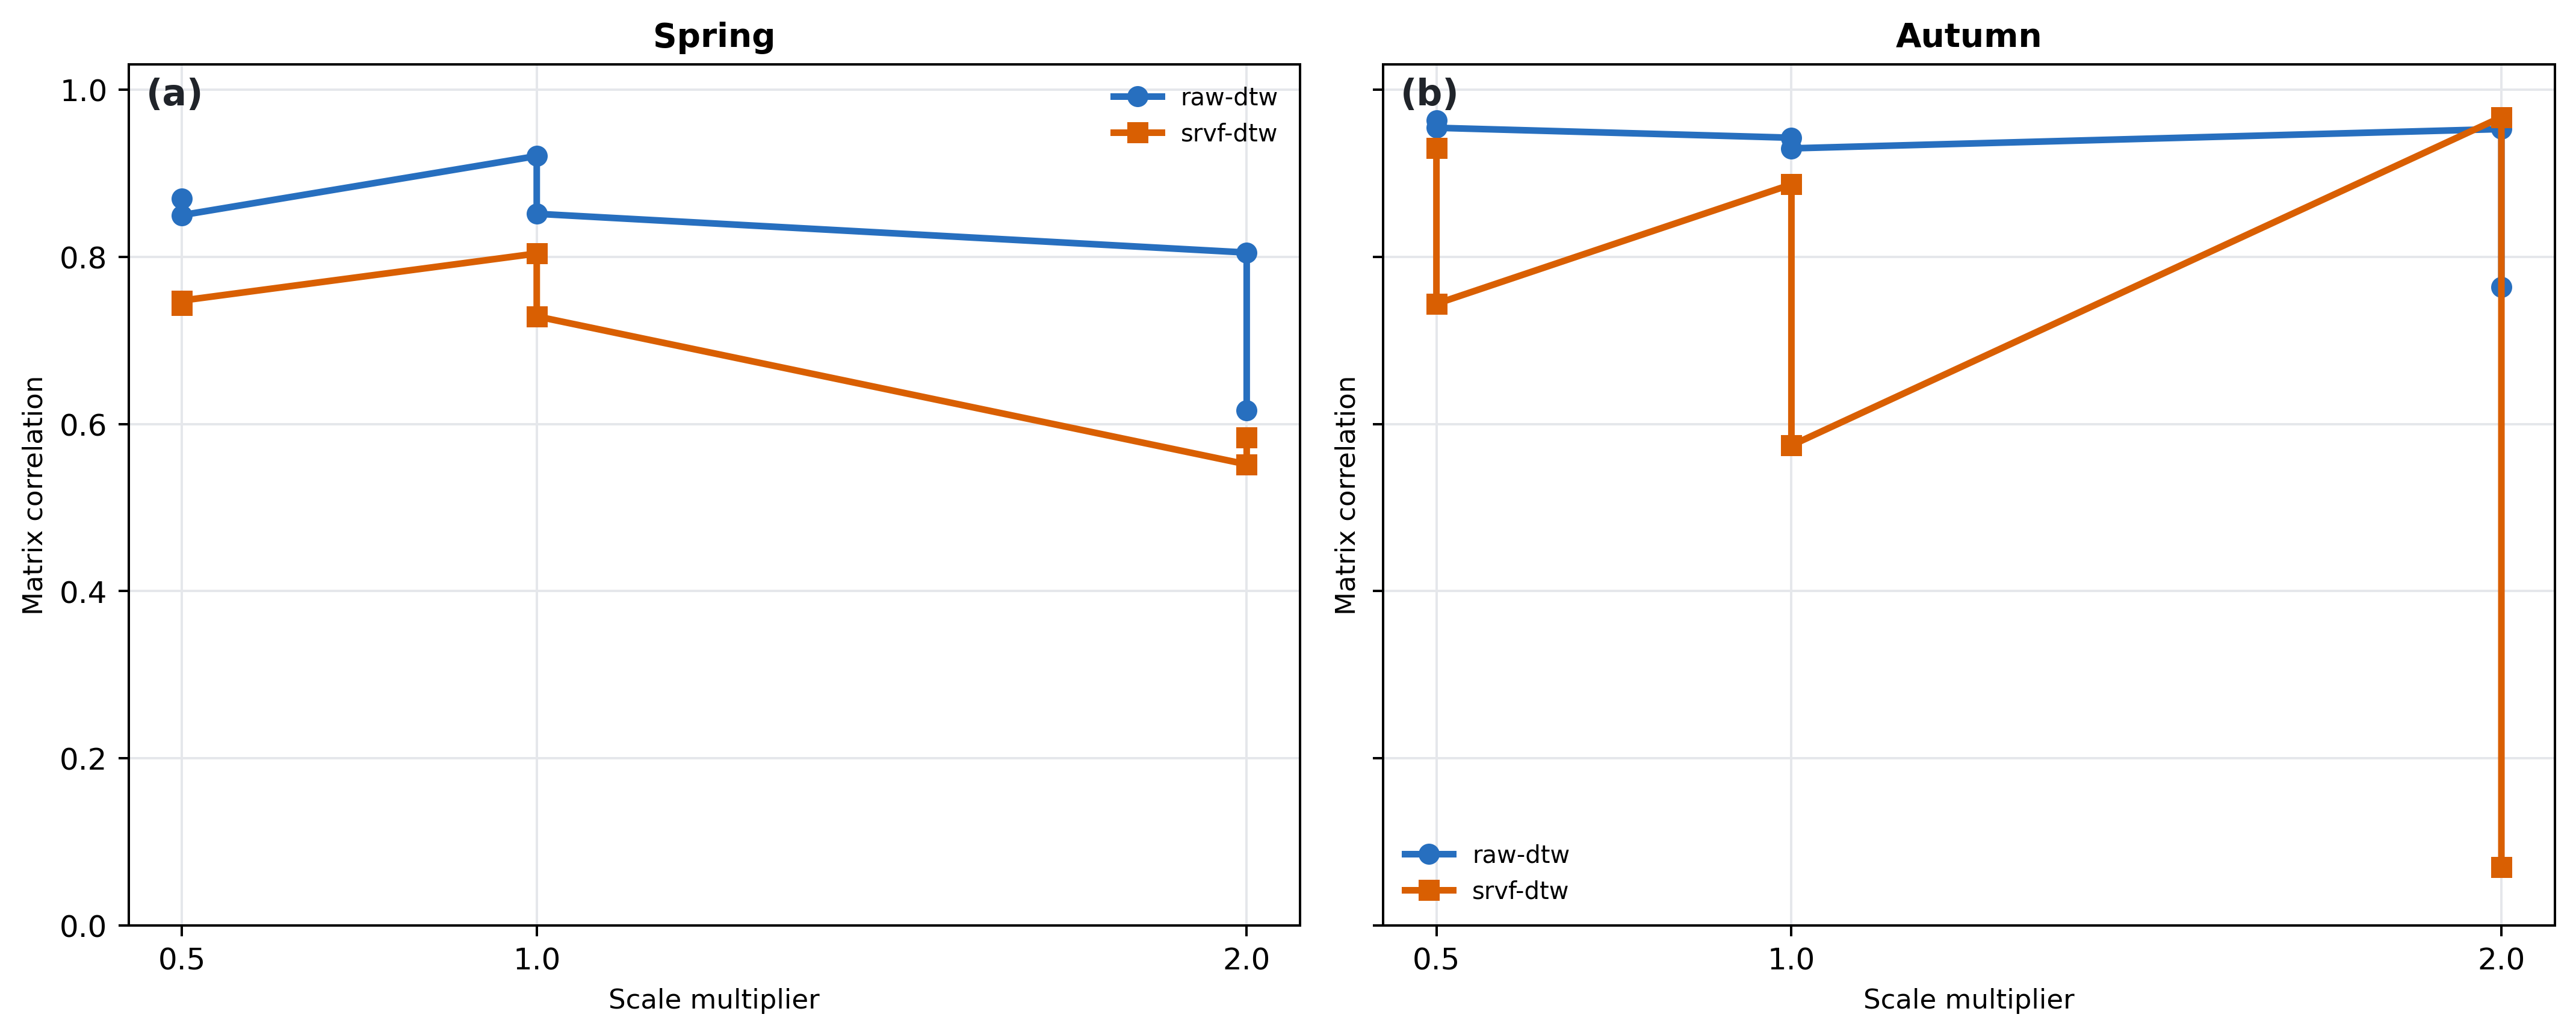
\includegraphics[width=0.95\textwidth]{../../figures/brownian_scale_sensitivity.png}
\caption{Sensitivity of route-distance stability to Brownian bridge perturbation scale at 60\% contiguous gaps. The estimated seasonal scale was multiplied by 0.5, 1.0, and 2.0; matrix correlations are shown separately for raw-DTW and SRVF-DTW distances.}
\label{fig:brownian-scale-sensitivity}
\end{figure}

\begin{table}[H]
\centering
\caption{Brownian bridge reconstruction diagnostics at 60\% contiguous gaps. Values are means across sampled reconstructions. Matrix correlation and anomaly correlation are Spearman correlations; relative error is the median relative distance error; ARI is adjusted Rand index for cluster labels.}
\label{tab:brownian-60}
\resizebox{\textwidth}{!}{%
\begin{tabular}{llrrrrrr}
\toprule
Season & Metric & Scale & Matrix corr. & Rel. error & ARI & Anomaly corr. & Top-k overlap \\
\midrule
Spring & Raw DTW & 0.001088 & 0.929 & 0.128 & 0.791 & 0.831 & 0.933 \\
Spring & SRVF-DTW & 0.001088 & 0.836 & 0.119 & 0.626 & 0.887 & 0.744 \\
Autumn & Raw DTW & 0.000352 & 0.958 & 0.115 & 0.878 & 0.931 & 0.733 \\
Autumn & SRVF-DTW & 0.000352 & 0.707 & 0.096 & 0.493 & 0.679 & 0.622 \\
\bottomrule
\end{tabular}
}
\end{table}

\begin{figure}[t]
\centering
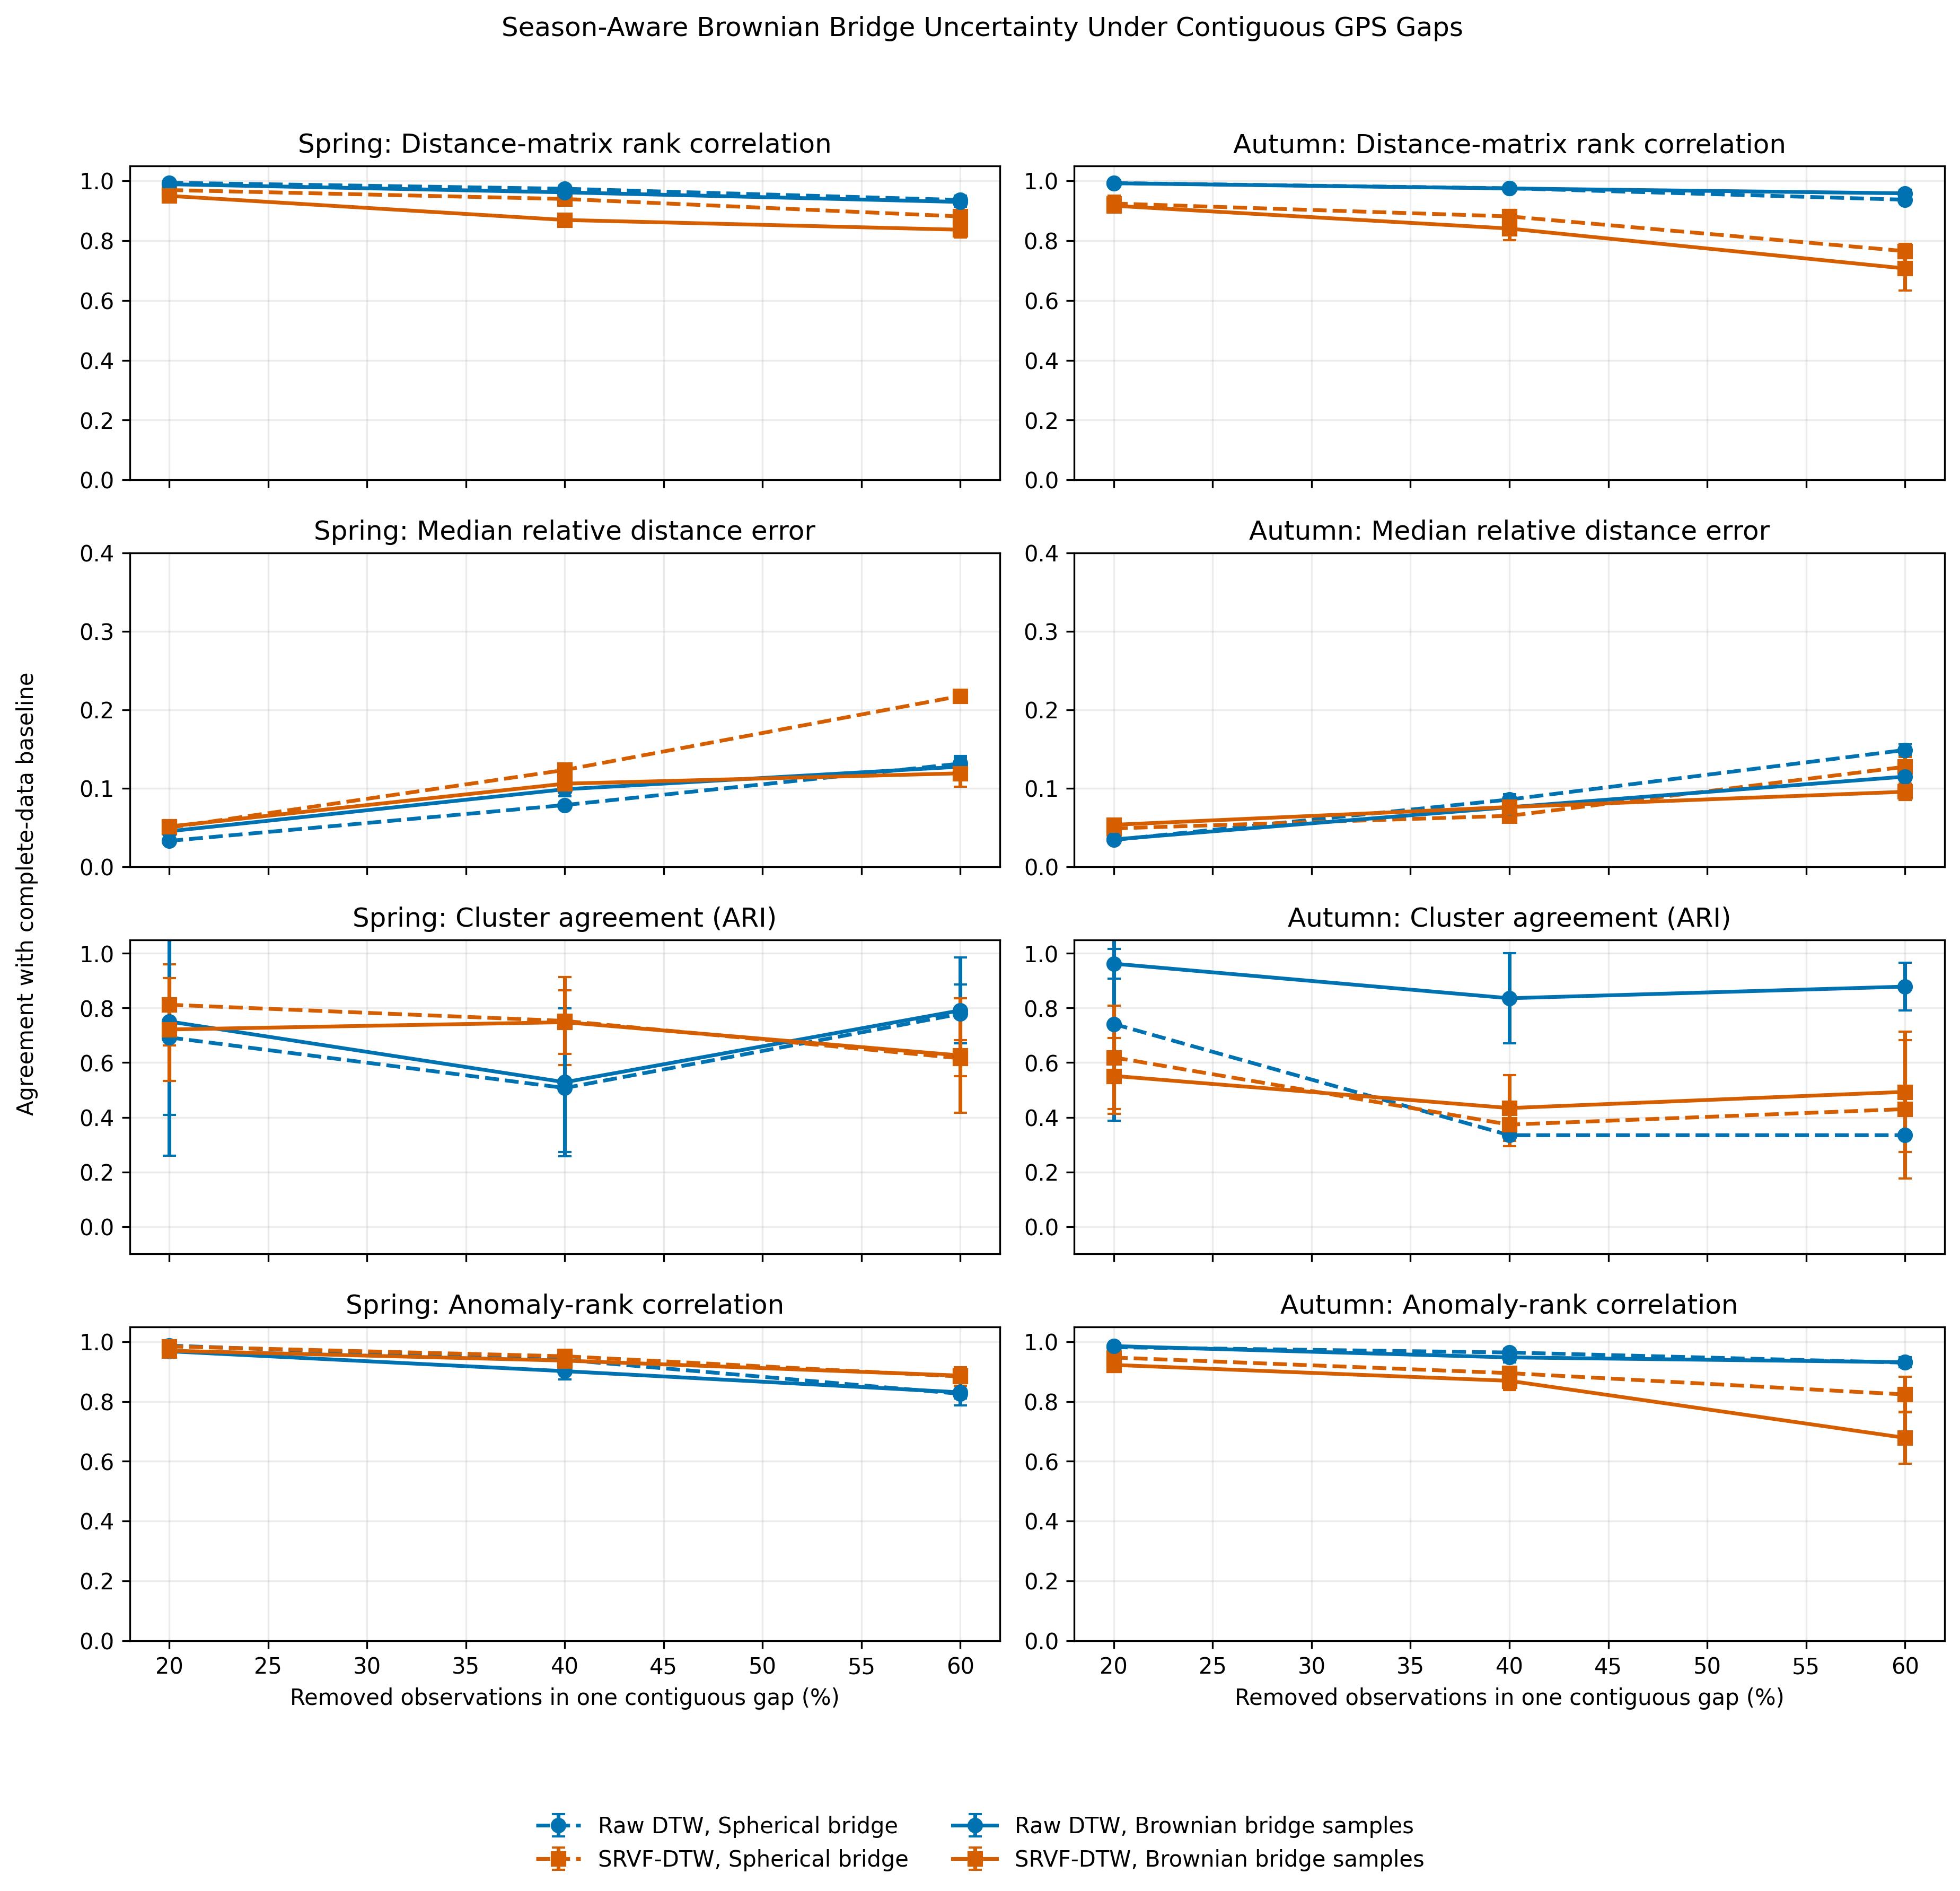
\includegraphics[width=\textwidth]{../../figures/brownian_bridge_gap_reconstruction_batch.png}
\caption{Season-aware Brownian bridge reconstruction diagnostics across gap fractions, metrics, and seasons. The experiment propagates sampled missing-route reconstructions into distance-matrix correlation, relative distance error, cluster agreement, anomaly-rank correlation, and top-ranked anomaly overlap.}
\label{fig:brownian-bridge-batch}
\end{figure}

\subsection{Withheld-Segment Validation}\label{withheld-segment-validation}

The withheld-segment validation showed that the Brownian bridge baseline should not be interpreted as a calibrated true-path reconstruction model. Table~\ref{tab:withheld-validation} summarizes the validation diagnostics. Deterministic spherical bridge mean error increased with withheld fraction, from 74.1 km to 171.2 km in spring and from 59.8 km to 140.8 km in autumn. The pointwise center of the Brownian bridge samples had similar mean error, ranging from 75.6 km to 172.8 km in spring and from 61.8 km to 143.8 km in autumn.

Brownian sampling did provide alternative plausible paths around the deterministic bridge, but the empirical 90\% envelope did not achieve nominal coverage of the withheld observations. Figure~\ref{fig:validation-calibration-summary} summarizes the withheld-segment errors and the effect of empirical radius inflation. Mean uncalibrated coverage ranged from 0.25 to 0.46 in spring and from 0.51 to 0.69 in autumn. The empirical calibration diagnostic estimated radius-inflation factors of 3.8 to 5.3 in spring and 6.5 to 8.0 in autumn, after which the calibrated pointwise coverage was approximately 0.89 to 0.90 across conditions. These results support the conservative interpretation of the Brownian bridge used in this paper: it is useful for stress-testing downstream route-comparison conclusions, but its uncertainty envelope should be validated and calibrated before being treated as a nominal coverage statement.

\begin{figure}[t]
\centering
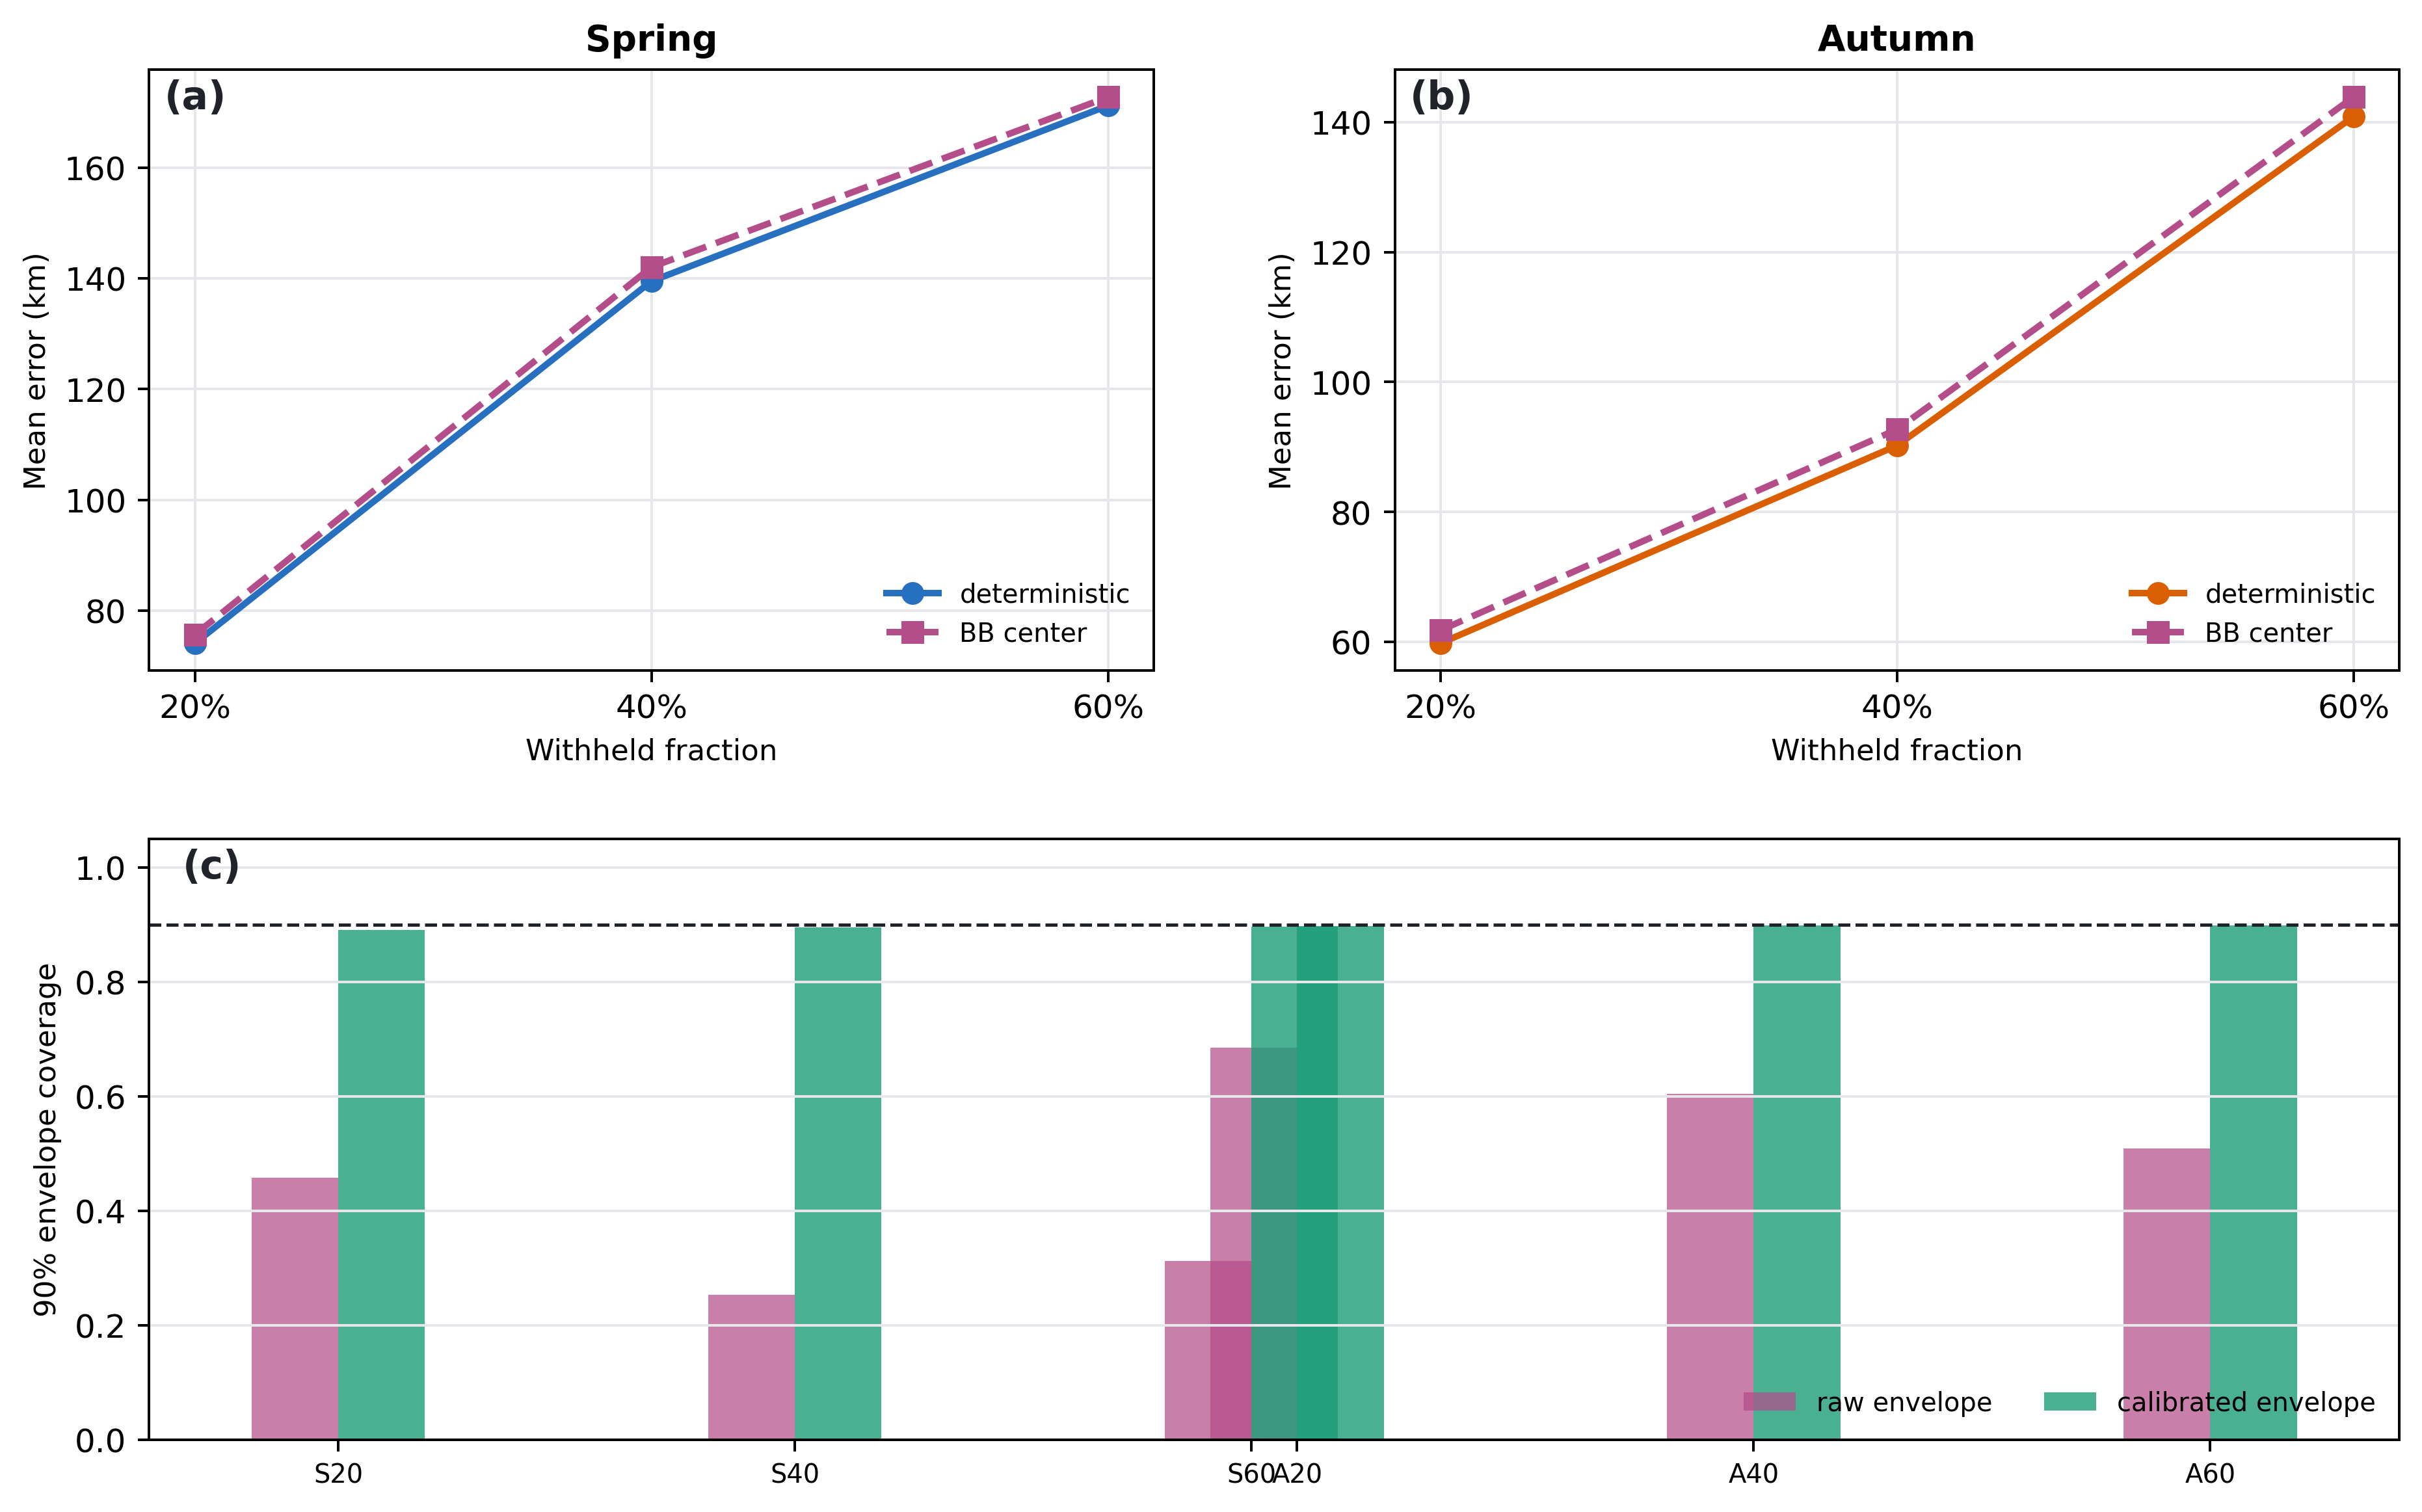
\includegraphics[width=\textwidth]{../../figures/validation_calibration_summary.png}
\caption{Withheld-segment validation and empirical envelope calibration. Mean reconstruction errors are shown for deterministic spherical bridges and Brownian bridge sample centers, while pointwise 90\% envelope coverage is compared before and after empirical radius inflation.}
\label{fig:validation-calibration-summary}
\end{figure}

\begin{table}[H]
\centering
\caption{Withheld-segment validation of deterministic spherical bridges and Brownian bridge samples. Errors are mean great-circle errors in kilometers. Coverage is the fraction of withheld observations falling inside the pointwise 90\% Brownian sample envelope. The inflation factor is the empirical multiplier required for approximately 90\% pointwise coverage.}
\label{tab:withheld-validation}
\small
\begin{tabular}{llrrrrr}
\toprule
Season & Gap & Det. err. & BB err. & Cover. & Infl. & Cal. cover. \\
\midrule
Spring & 20\% & 74.1 & 75.6 & 0.46 & 3.8 & 0.89 \\
Spring & 40\% & 139.5 & 142.0 & 0.25 & 4.4 & 0.89 \\
Spring & 60\% & 171.2 & 172.8 & 0.31 & 5.3 & 0.90 \\
Autumn & 20\% & 59.8 & 61.8 & 0.69 & 7.0 & 0.90 \\
Autumn & 40\% & 90.2 & 92.7 & 0.60 & 6.5 & 0.90 \\
Autumn & 60\% & 140.8 & 143.8 & 0.51 & 8.0 & 0.90 \\
\bottomrule
\end{tabular}
\end{table}

\section{Discussion}\label{discussion}

The results support the central claim that incomplete tracking data affect route-comparison conclusions through more than sampling density alone. Randomly missing observations were mostly absorbed by resampling, but contiguous gaps changed route distances, cluster labels, and anomaly rankings. This distinction matters because real tracking interruptions often occur as prolonged gaps rather than independent random point loss.

The study also shows why deterministic preprocessing is not enough. A spherical bridge supplies a single smooth path through a missing interval, but it does not represent uncertainty about the route that might have been taken. Downstream analyses based on that one path can therefore understate uncertainty. The Brownian bridge baseline provides a simple way to make this uncertainty visible by carrying multiple plausible reconstructed routes through the same distance and clustering workflow.

The most important practical result is that stability is task dependent. Distance-matrix rank correlations can remain high while cluster labels change substantially. Anomaly rankings can be more stable than clusters in some settings but less stable under severe season-specific gaps. For ecological informatics, this means that reporting one trajectory distance matrix is not sufficient when tracking gaps are long. Analysts should also report whether the conclusions drawn from that matrix are stable under plausible reconstruction uncertainty.

The Brownian bridge model used here should be interpreted conservatively. It is movement-aware in the limited sense that samples are local perturbations around a spherical bridge and the perturbation scale is estimated from observed route residuals. It is not a full continuous-time state-space model and does not use environmental covariates, behavioral states, wind fields, or stopover dynamics. The withheld-segment validation reinforces this interpretation: the sampled envelopes did not provide nominal 90\% coverage of the hidden observations without empirical radius inflation. The model's value is therefore as a transparent uncertainty baseline that can be validated, calibrated, and compared against richer movement models in future work.

The scale-sensitivity check also shows why the Brownian bridge should not be used as a single definitive reconstruction. Larger perturbation scales can substantially change downstream route-comparison diagnostics, especially for SRVF-DTW in autumn routes. This is a limitation of the simple scale estimator, but it is also the point of the proposed workflow: reconstruction assumptions should be propagated and reported rather than hidden inside one completed trajectory table.

The present analysis should therefore be read primarily as a downstream stability study, not as a claim that the Brownian bridge recovers the true unobserved route. The complete-data baseline is used to ask whether route-comparison conclusions change after observations are removed and reconstructed. The added withheld-segment validation and radius-inflation diagnostic provide a direct check on reconstructed path geometry and nominal coverage, but a stronger reconstruction-validation study would require more repeated gap locations, temporal sampling regimes, explicit location error, and comparisons with continuous-time or state-space movement models.

Several limitations remain. First, the empirical analysis uses one species and one public tracking dataset. Second, migration segmentation is heuristic and should not be interpreted as validated behavioral-state classification. The threshold sensitivity check shows that route counts are stable under moderate trimming changes, but it does not validate biological departure or arrival times. Third, the Brownian bridge scale estimator is simple; the lightweight withheld validation indicates that it is not fully calibrated, and the scale-sensitivity check shows that downstream diagnostics can change under scale inflation. Fourth, the cluster and anomaly diagnostics do not have external ecological labels, so they measure computational stability rather than biological correctness. Fifth, the current experiment varies gap fraction but does not yet fully vary gap location, temporal sampling interval, or location error.

This single-dataset design limits biological generalization but not the methodological point of the paper. The empirical numbers should be read as properties of the \texttt{LBBG\_ZEEBRUGGE} case study. The workflow itself is dataset-agnostic and can be applied to other movement datasets wherever routes, gaps, reconstruction assumptions, and downstream comparison tasks can be specified.

Future work should extend this framework to additional tracking datasets and richer reconstruction models. Continuous-time movement models, state-space models \citep{patterson2008}, environmental conditioning, and explicit stopover behavior could all provide more realistic missing-route distributions. The key requirement is that such models should not stop at reconstructing tracks; they should propagate reconstruction uncertainty into the ecological or computational conclusions that depend on trajectory distances.

\section{Conclusion}\label{conclusion}

This study reframes migratory-route comparison as an uncertainty-propagation problem under incomplete tracking data. In a reproducible open-data case study of Lesser Black-backed Gulls, random point loss had limited influence after resampling, whereas contiguous gaps substantially affected route-comparison diagnostics. Deterministic bridge interpolation did not fully resolve this instability. An estimated-scale Brownian bridge provided a practical uncertainty-aware baseline, withheld-segment validation showed that its nominal envelope required empirical calibration, and downstream stability varied by season, metric, and analytical task. These findings support reporting calibrated uncertainty-aware diagnostics whenever route distances are used for clustering, anomaly screening, or other ecological movement-data conclusions.
